\documentclass{article}


\usepackage{amsmath}
\usepackage{amssymb}
\usepackage{cancel}
\usepackage{graphicx}
\usepackage{float}
\usepackage{subcaption}
\usepackage{matlab-prettifier}
\usepackage[margin=1.0in]{geometry}




% bold letters
\newcommand{\bola}{\mathbf{a}}
\newcommand{\bolc}{\mathbf{c}}
\newcommand{\bolf}{\mathbf{f}}
\newcommand{\bolg}{\mathbf{g}}
\newcommand{\boll}{\mathbf{l}}
\newcommand{\bolq}{\mathbf{q}}
\newcommand{\bolp}{\mathbf{p}}
\newcommand{\bolu}{\mathbf{u}}
\newcommand{\bolv}{\mathbf{v}}
\newcommand{\bolw}{\mathbf{w}}
\newcommand{\bolz}{\mathbf{z}}

\newcommand{\bolA}{\mathbf{A}}
\newcommand{\bolB}{\mathbf{B}}
\newcommand{\bolC}{\mathbf{C}}
\newcommand{\bolD}{\mathbf{D}}
\newcommand{\bolE}{\mathbf{E}}
\newcommand{\bolF}{\mathbf{F}}
\newcommand{\bolG}{\mathbf{G}}
\newcommand{\bolH}{\mathbf{H}}
\newcommand{\bolI}{\mathbf{I}}
\newcommand{\bolJ}{\mathbf{J}}
\newcommand{\bolK}{\mathbf{K}}
\newcommand{\bolL}{\mathbf{L}}
\newcommand{\bolM}{\mathbf{M}}
\newcommand{\bolN}{\mathbf{N}}
\newcommand{\bolO}{\mathbf{O}}
\newcommand{\bolP}{\mathbf{P}}
\newcommand{\bolQ}{\mathbf{Q}}
\newcommand{\bolR}{\mathbf{R}}
\newcommand{\bolS}{\mathbf{S}}
\newcommand{\bolT}{\mathbf{T}}
\newcommand{\bolU}{\mathbf{U}}
\newcommand{\bolV}{\mathbf{V}}
\newcommand{\bolW}{\mathbf{W}}
\newcommand{\bolX}{\mathbf{X}}
\newcommand{\bolY}{\mathbf{Y}}
\newcommand{\bolZ}{\mathbf{Z}}

% bold symbols
\newcommand{\bolalpha}{\boldsymbol{\alpha}}
\newcommand{\bolbeta}{\boldsymbol{\beta}}
\newcommand{\boleta}{\boldsymbol{\eta}}
\newcommand{\bolpsi}{\boldsymbol{\psi}}

% shadowed letters
\newcommand{\PP}{\mathbb{P}}
\newcommand{\RR}{\mathbb{R}}
\newcommand{\CC}{\mathbb{C}}
\newcommand{\ZZ}{\mathbb{Z}}

% mathcal letters
\newcommand{\calA}{\mathcal{A}}
\newcommand{\calB}{\mathcal{B}}
\newcommand{\calC}{\mathcal{C}}
\newcommand{\calD}{\mathcal{D}}
\newcommand{\calE}{\mathcal{E}}
\newcommand{\calF}{\mathcal{F}}
\newcommand{\calG}{\mathcal{G}}
\newcommand{\calH}{\mathcal{H}}
\newcommand{\calI}{\mathcal{I}}
\newcommand{\calJ}{\mathcal{J}}
\newcommand{\calK}{\mathcal{K}}
\newcommand{\calL}{\mathcal{L}}
\newcommand{\calM}{\mathcal{M}}
\newcommand{\calN}{\mathcal{N}}
\newcommand{\calO}{\mathcal{O}}
\newcommand{\calP}{\mathcal{P}}
\newcommand{\calQ}{\mathcal{Q}}
\newcommand{\calR}{\mathcal{R}}
\newcommand{\calS}{\mathcal{S}}
\newcommand{\calT}{\mathcal{T}}
\newcommand{\calU}{\mathcal{U}}
\newcommand{\calV}{\mathcal{V}}
\newcommand{\calW}{\mathcal{W}}
\newcommand{\calX}{\mathcal{X}}
\newcommand{\calY}{\mathcal{Y}}
\newcommand{\calZ}{\mathcal{Z}}


% derivatives
\newcommand{\pp}[2]{\frac{\partial #1}{\partial #2}}
\newcommand{\dd}[2]{\frac{d #1}{d #2}}


% fraction shortcut
\newcommand{\f}[2]{\frac{#1}{#2}}
\newcommand{\slfrac}[2]{\left.#1\middle/#2\right.}

% common operators
\newcommand{\vvvert}{|\kern-1pt|\kern-1pt|}
\newcommand{\enorm}[1]{\vvvert #1 \vvvert}


% matrices
\newcommand{\bmat}[1]{\left(\begin{array}{#1}}
\newcommand{\emat}{\end{array}\right)} 



\newcommand{\blist}{\begin{list}{\ballrefb}{\leftmargin=2.0em}
  \setlength{\itemsep}{2pt}
  \setlength{\parskip}{0pt}}
\newcommand{\elist}{\end{list}}



% common format strings
\def\etal{{\it et al.}}
\def\ie{{\it i.e.}}
\def\eg{{\it e.g.}}


\DeclareMathOperator*{\arginf}{arg\,inf}
\DeclareMathOperator*{\argsup}{arg\,sup}
\DeclareMathOperator*{\argmax}{arg\,max}
\DeclareMathOperator*{\argmin}{arg\,min}


\begin{document}
\Large\centering AER1418: Assignment 4\\
\normalsize\raggedright Geoff Donoghue \hfill April 26, 2019\\

\section*{Part 1. Advection-diffusion equation}
\begin{itemize}
	\item[(a)] We wish to show that \(\exists\gamma < \infty \) such that
	\begin{equation*}
		a_h(w,v) \equiv a(w,v) + \left(\tau\calL w, \calL v \right)_{L^2(\Omega)} \leq \gamma\|w\|_{\calV_h}\|v\|_{\calV_h}, \quad \forall w,v\in \calV_h.
	\end{equation*}
	Since we already know that
	\begin{equation*}
		a(w,v) \leq \left(\|\kappa\|_{L^\infty(\Omega)} + \|b\|_{L^\infty(\Omega)} + C^2_\text{tr}\|b\|_{L^\infty(\Gamma_N)} \right)\|w\|_{\calV_h}\|v\|_{\calV_h},
	\end{equation*}
	we seek some \(\gamma' < \infty \) such that
	\begin{equation*}
		\left(\tau\calL w, \calL v \right)_{L^2(\Omega)} \leq \gamma'\|w\|_{\calV_h}\|v\|_{\calV_h}, \quad \forall w,v\in \calV_h.
	\end{equation*}
	We first apply the Cauchy-Schwarz inequality to the leas-squares term, obtaining
	\begin{equation*}
		\left(\tau\calL w, \calL v \right)_{L^2(\Omega)} \leq \|\tau\calL w\|_{L^2(\Omega)}\|\calL v\|_{L^2(\Omega)}.
	\end{equation*}
	Now using the definition of \(\calL \), we can say that
	\begin{equation*}
		\left(\tau\calL w, \calL v \right)_{L^2(\Omega)} \leq \|\tau(-\nabla\cdot(\kappa\nabla w) + \nabla\cdot(bw))\|_{L^2(\Omega)}\|-\nabla\cdot(\kappa\nabla v) + \nabla\cdot(bv)\|_{L^2(\Omega)}.
	\end{equation*}
	By applying the triangle inequality to the norms containing sums we arrive at
	\begin{equation*}
		\left(\tau\calL w, \calL v \right)_{L^2(\Omega)} \leq (\|-\tau\nabla\cdot(\kappa\nabla w)\|_{L^2(\Omega)} + \|\tau\nabla\cdot(bw)\|_{L^2(\Omega)})(\|-\nabla\cdot(\kappa\nabla v)\|_{L^2(\Omega)} + \|\nabla\cdot(bv)\|_{L^2(\Omega)}).
	\end{equation*}
	If we assume that our advection and diffusion fields are constant we may reexpress the above as
	\begin{equation*}
		\left(\tau\calL w, \calL v \right)_{L^2(\Omega)} \leq \tau(\kappa\|\nabla^2 w\|_{L^2(\Omega)} + b\cdot\|\nabla w\|_{L^2(\Omega)})(\kappa\|\nabla^2 v\|_{L^2(\Omega)} + b\cdot\|\nabla v\|_{L^2(\Omega)}).
	\end{equation*}
	Using the definitions of the \(H^2(\Omega) \) and \(H^1(\Omega) \) semi-norms we can say that
	\begin{equation*}
		\left(\tau\calL w, \calL v \right)_{L^2(\Omega)} \leq \tau(\kappa|w|_{H^2(\Omega)} + b\cdot| w|_{H^1(\Omega)})(\kappa|v|_{H^2(\Omega)} + b\cdot|v|_{H^1(\Omega)}).
	\end{equation*}
	Since we have \(\calV_h \subset H^1(\Omega) \), \(\overline{\Omega} = \bigcup_{K\in\calT_h}\overline{K}\), and we assume the inverse esimtate estmate \(|v|_{H^2(K)} \leq c_\text{inv}h^{-1}\|v\|_{H^1(K)} \forall v \in \calV_h \) our inequality now becomes
	\begin{equation*}
		\left(\tau\calL w, \calL v \right)_{L^2(\Omega)} \leq \tau\Sigma_{K\in\calT_h}(\kappa c_\text{inv}h^{-1}\|w\|_{H^1(K)} + b\cdot| w|_{H^1(\Omega)})(\kappa c_\text{inv}h^{-1}\|v\|_{H^1(K)} + b\cdot|v|_{H^1(\Omega)}).
	\end{equation*}
	From the definition of the \(H^1(\Omega) \) seminorm, \(\|v\|_{H^1(\Omega)} \equiv \|v\|_{L^2(\Omega)} + |v|_{H^1(\Omega)}, \; \forall v \in H^1(\Omega) \), we note that by the non-negativity of \(\|v\|_{L^2(\Omega)} \) implies that \(\|v\|_{H^1(\Omega)} \geq |v|_{H^1(\Omega)} \), applying this to our inequality we arrive at
	\begin{equation*}
		\left(\tau\calL w, \calL v \right)_{L^2(\Omega)} \leq \tau\Sigma_{K\in\calT_h}(\kappa c_\text{inv}h^{-1}\|w\|_{H^1(K)} + b\cdot\| w\|_{H^1(\Omega)})(\kappa c_\text{inv}h^{-1}\|v\|_{H^1(K)} + b\cdot\|v\|_{H^1(\Omega)}).
	\end{equation*}
	\begin{equation*}
		\left(\tau\calL w, \calL v \right)_{L^2(\Omega)} \leq \tau\Sigma_{K\in\calT_h}(\kappa c_\text{inv}h^{-1}+b)\|w\|_{H^1(K)} (\kappa c_\text{inv}h^{-1} + b)\|v\|_{H^1(K)}.
	\end{equation*}
	Since when we invoked the inverse estimate inequality, we can now express \(\tau\) in the limit as \(h \to 0 \), which is \(\tau = \dfrac{h^2}{12\kappa} \), this updates our inequality to become
	\begin{equation*}
		\left(\tau\calL w, \calL v \right)_{L^2(\Omega)} \leq \frac{h^2}{12\kappa}(\kappa c_\text{inv}h^{-1}+b)^2 \Sigma_{K\in\calT_h} \|w\|_{H^1(K)} \|v\|_{H^1(K)}.
	\end{equation*}
	Since \(h \to 0\) the only term that survives is
	\begin{equation*}
		\left(\tau\calL w, \calL v \right)_{L^2(\Omega)} \leq \frac{\kappa}{12}c_\text{inv}^2 \|w\|_{H^1(\Omega)} \|v\|_{H^1(\Omega)}.
	\end{equation*}
	Therefore we say that the bilinear form of the advection-diffusion equation arising from the GLS discretization is continuous with a continuity constant
	\begin{equation*}
		\gamma = \|\kappa\|_{L^\infty(\Omega)} + \|b\|_{L^\infty(\Omega)} + C^2_\text{tr}\|b\|_{L^\infty(\Gamma_N)} + \frac{\kappa}{12}c_\text{inv}^2.
	\end{equation*}
	
	\item[(b)] Assuming a constant diffusion field, our problem is given by
	\begin{equation*}
		-\kappa\left(\dfrac{\partial^2u}{\partial x_1^2} + \dfrac{\partial^2u}{\partial x_2^2} \right) + \pp{u}{x_1} = 0.
	\end{equation*}
	We note that this problem is separable and express our solution as the product of monomial functions \(u = X_1X_2 \) and obtain
	\begin{equation*}
		-\kappa\dfrac{1}{X_1}\dfrac{d^2X_1}{dx_1^2} + \dfrac{1}{X_1}\dd{X_1}{x_1} = \kappa \dfrac{1}{X_2}\dfrac{d^2X_2}{dx_2^2} = m,
	\end{equation*}
	where \(m\) is some seperation constant. The ordinary differential equation in \(x_2 \),
	\begin{equation*}
		\dfrac{d^2X_2}{dx_2^2} = \dfrac{m}{\kappa}X_2,
	\end{equation*}
	is trivial to solve; the solution is given by
	\begin{equation*}
		X_2(x_2) = c_1\exp\left(\sqrt{\frac{m}{\kappa}}x_2\right) + c_2\exp\left(-\sqrt{\frac{m}{\kappa}}x_2\right).
	\end{equation*}
	Our boundary conditions state that
	\begin{equation*}
		\left.\dd{X_2}{x_2}\right|_{x_2 = 0} = 0 = c_1\sqrt{\dfrac{m}{\kappa}} - c_2\sqrt{\dfrac{m}{\kappa}} \implies c_1 = c_2,
	\end{equation*}
	\begin{equation*}
		\left.\dd{X_2}{x_2}\right|_{x_2 = 1} = 0 = c_1\sqrt{\dfrac{m}{\kappa}}\exp\left(\sqrt{\frac{m}{\kappa}}\right) - c_1\sqrt{\dfrac{m}{\kappa}}\exp\left(-\sqrt{\frac{m}{\kappa}}\right) \implies c_1 \vee m = 0.
	\end{equation*}
	Since either \(c_1\) or \(m\) will result in the trivial solution, we will take \(m=0\) and see if the resulting solution for \(u\) satisfies our differential equation, then invoke Lax-Milgram to justify the uniqueness of the solution. By taking \(m\) to be zero, our ordinary differential equation in \(x_2\) is updated to become
	\begin{equation*}
		\dfrac{d^2X_2}{dx^2} = 0, \quad \left.\dd{X_2}{x_2}\right|_{x_2 = 0} = 0, \quad \left.\dd{X_2}{x_2}\right|_{x_2 = 1} = 0.
	\end{equation*}
	Here we note that any constant function will satisfy all of these equations, the magnitude of this constant can be absorbed into \(X_1\) and we will therefore say that \(X_2 = 1\).

	Our ordinary differential equation in \(x_1\) is then given by
	\begin{equation*}
		-\kappa\dfrac{d^2X_1}{dx_1^2} + \dd{X_1}{x_1} = 0, \quad X_1(x_1 = 0) = 1, \quad X_1(x_1 = 1) = 0,
	\end{equation*}
	which has the characteristic equation
	\begin{equation*}
		-\kappa r^2 + r = 0, \implies r = \dfrac{1}{\kappa}.
	\end{equation*}
	Assuming a solution given by a linearly independent combination of exponentials, we can apply our boundary conditions to obtain
	\begin{equation*}
		X_1(x_1) = \dfrac{e^{x_1/\kappa} - e^{1/\kappa}}{1 - e^{1/\kappa}}.
	\end{equation*}
	The closed form solution of our advection-diffusion equation is 
	\begin{equation*}
	u(x_1,x_2;\kappa) = X_1(x_1;\kappa)X_2(x_2) = \dfrac{e^{x_1/\kappa} - e^{1/\kappa}}{1 - e^{1/\kappa}}.
	\end{equation*}
	
	\item[(c-f)] See appendix.
	
	\item[(g)]  The standard continuous Galerkin and Galerkin least-squares solution fields for the above equation using a \(\PP^2 \) approximation are shown in Figue \ref{fig:addiff-test_solns}.
	\begin{figure}[H]
		\centering
		\begin{subfigure}[b]{0.48\textwidth}
			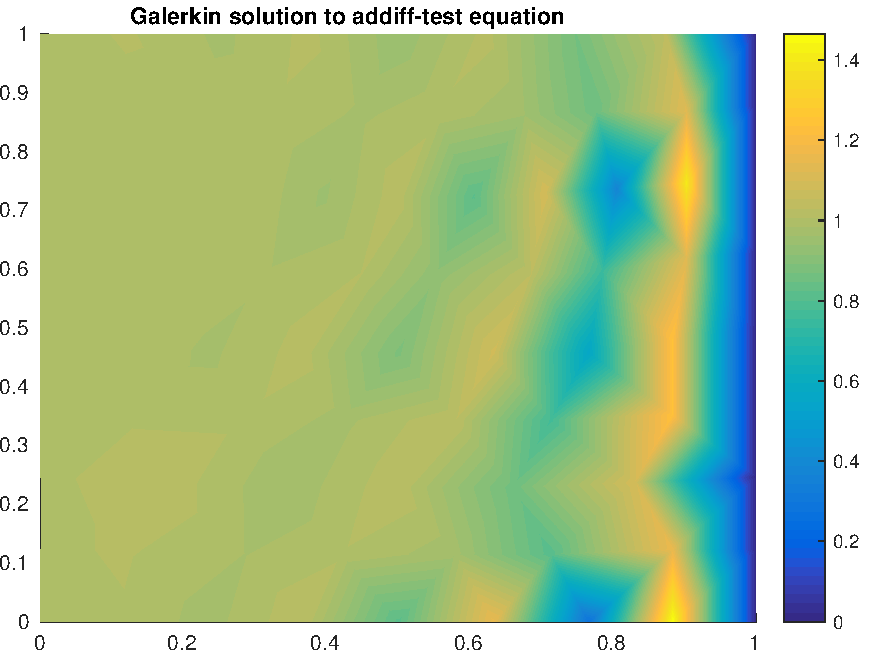
\includegraphics[width=\textwidth]{addiff-test_soln_Galerkin.pdf}
			\caption{Without GLS Stabilization}
		\end{subfigure}
		\begin{subfigure}[b]{0.48\textwidth}
			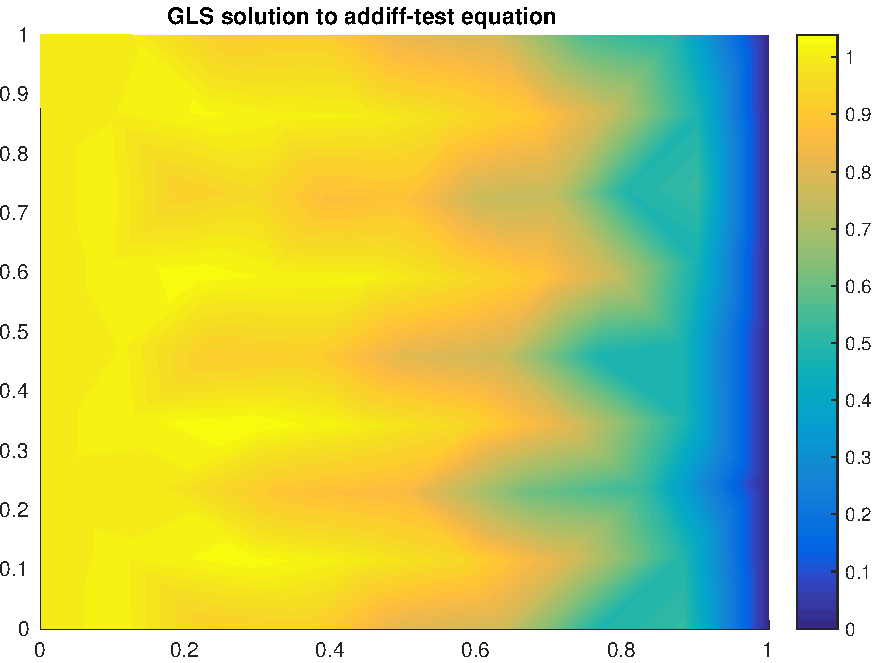
\includegraphics[width=\textwidth]{addiff-test_soln_GLS.pdf}
			\caption{With GLS Stabilization}
		\end{subfigure}
		\caption{Galerkin approximations to the advection-diffusion test equation.}
		\label{fig:addiff-test_solns}
	\end{figure}
	We note qualitatively for now that the unstabilized method has a maximum overshoot that is greatly reduced by applying Galerkin least-squares stabilization. \\
	
	The convergence of the \(L^2(\Omega)\) norm of the solution error is shown in Figure \ref{fig:addiff-test_conv} below.
	\begin{figure}[H]
		\centering
		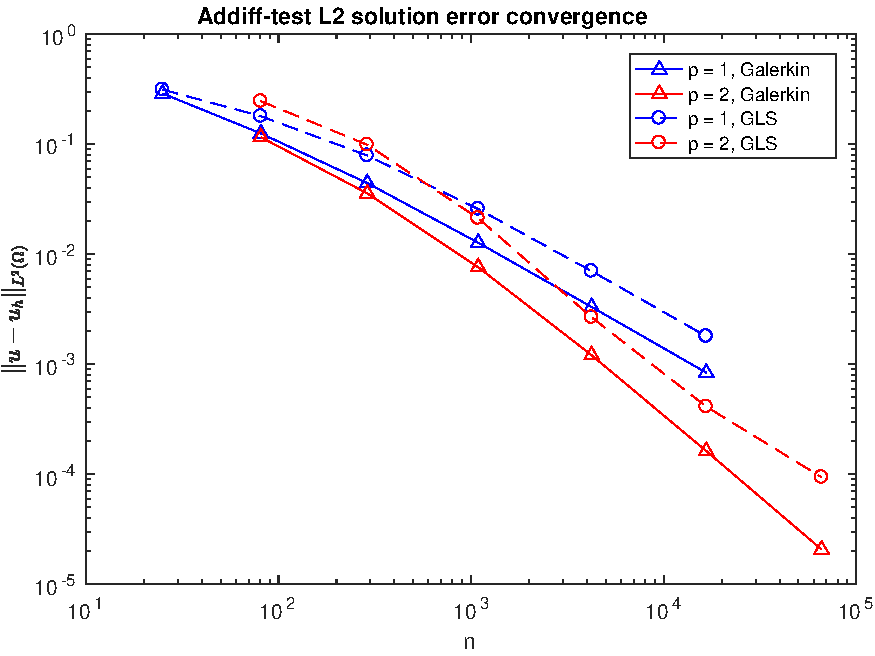
\includegraphics[width=0.65\textwidth]{addiff-test_conv_2.pdf}
		\caption{\(L^2(\Omega)\) error convergence, \(\PP^1\), and \(\PP^2 \)}
		\label{fig:addiff-test_conv}
	\end{figure}
	The asymptotic convergence rates for each scheme are summarized in table \ref{tab:addiff-test_conv}. We note that the expected convergence rates with respect to the \(n\) for the \(L^2(\Omega)\) norm of the error are \(h^{p+1} \sim n^{-(p+1)/2} \). Moreover, for the GLS scheme we expect a supoptimal convergence for the \(L^2(\Omega)\) norm of the error \(\sim n^{-(p+1/2)/2} \) but we may hope to recover the optimal convergence rate for this problem if it is sufficiently smooth.
	\begin{table}[H]
		\centering
		\begin{tabular}{r||c|c}
			& \(\PP^1 \) & \(\PP^2 \) \\
			\hline
			Expected Galerkin & -1.00 & -1.50 \\
			\hline
			Expected GLS & -1.00 & -1.50 \\
			\hline
			Actual Galerkin & -0.9975 & -1.4789 \\
			\hline
			Actual GLS & -0.9768 & -1.3638 \\

		\end{tabular}
		\caption{Convergence rates for each of the schemes.}
		\label{tab:addiff-test_conv}
	\end{table}
	Here we note that all of the convergence rates are in good agreement with the expected finite element theory, and that the true solution is apparently smooth enough to yield the optimal convergence rate for GLS.\\
	
	Lastly, we consider the maximum overshoot in the FE coefficients, these results are shown in Figure \ref{fig:addiff-test_maxover}. 
	\begin{figure}[H]
		\centering
		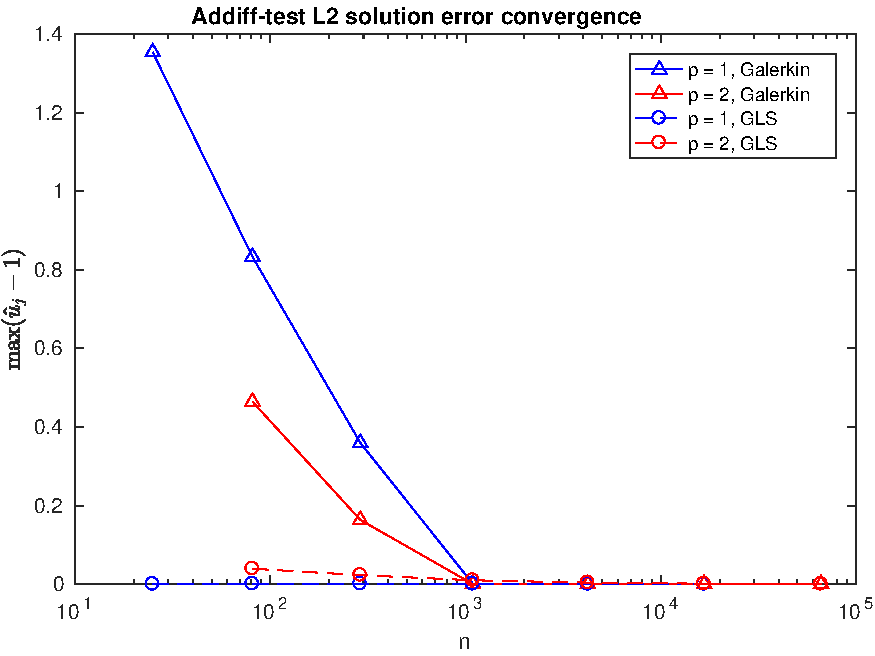
\includegraphics[width=0.65\textwidth]{addiff-test_maxover.pdf}
		\caption{Maximum overshoot, for standard Galerkin and GLS with \(\PP^1\) and \(\PP^2 \)}
		\label{fig:addiff-test_maxover}
	\end{figure}
	It is clear that the stability term introduced by GLS greatly reduces the maximum overshoot for coarse meshes. This difference becomes minimized as the mesh is refined.
	
	
\end{itemize}

\clearpage
\section*{Part 2. Error estimation and adaptive mesh refinement}
\begin{itemize}
	\item[(a)] See appendix.
	
	\item[(b)] Adaptive convergence plots for the test advection-diffusion problem are shown in Figure \ref{fig:21}.
	\begin{figure}[H]
		\centering
		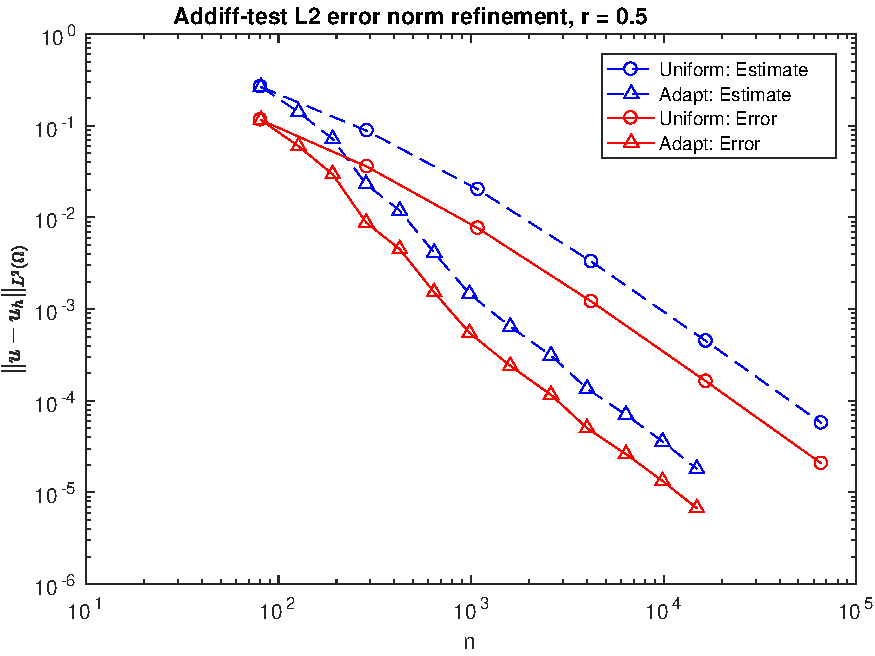
\includegraphics[width=0.65\textwidth]{addiff-test_adapt.pdf}
		\caption{This is a caption. r = 0.5}
		\label{fig:21}
	\end{figure}
	The convergence rates are showin in Table \ref{tab:21}.
	\begin{table}[H]
		\centering
		\begin{tabular}{r||c|c}
			& Uniform & Adaptive \\
			\hline
			Expected & -1.50 & -1.50 \\
			\hline
			Actual & -1.4925 & -1.6017 \\
			
		\end{tabular}
		\caption{Convergence rates for the uniform and adaptive refinement algorithms.}
		\label{tab:21}
	\end{table}
	The rate parameter used for the error estimates was \(r = 1/2\), in order to justify this we can consider the error estimates using other rate parameters \(r = 1, r = 2\). These results are shown in Figure \ref{fig:22} below.
	\begin{figure}[H]
		\centering
		\begin{subfigure}[b]{0.48\textwidth}
			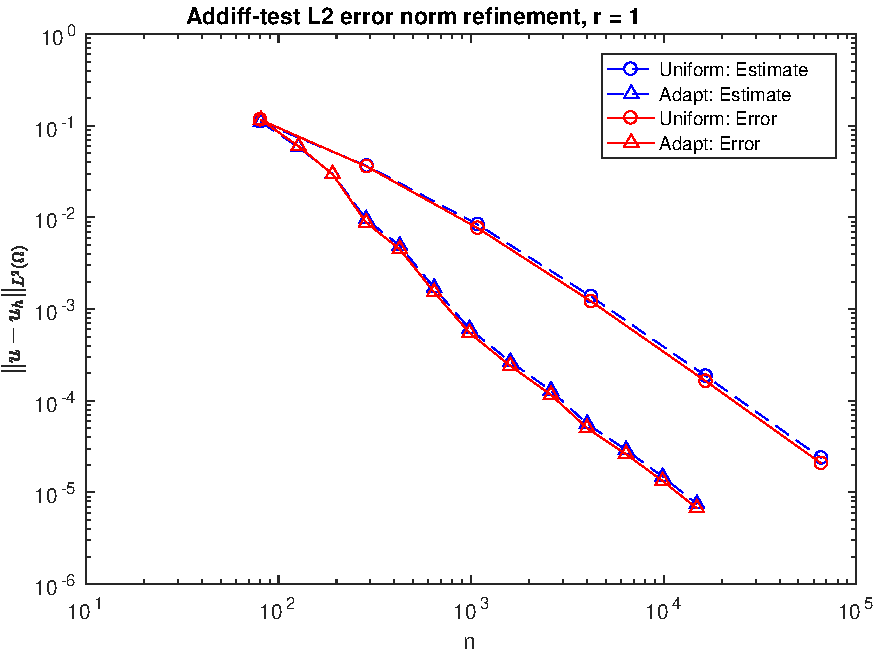
\includegraphics[width=\textwidth]{addiff-test_adapt_r1.pdf}
			\caption{\(r = 1\)}
		\end{subfigure}
		\begin{subfigure}[b]{0.48\textwidth}
			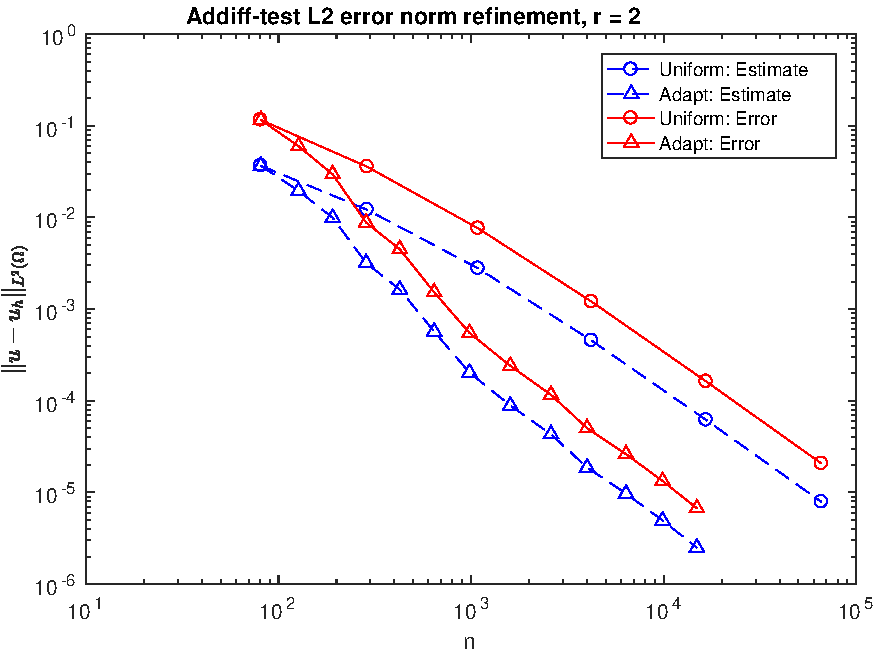
\includegraphics[width=\textwidth]{addiff-test_adapt_r2.pdf}
			\caption{\(r = 2\)}
		\end{subfigure}
		\caption{Convergence of Galerkin and GLS schemes for \(r=1\), and \(r=2 \).}
		\label{fig:22}
	\end{figure}
	We see that for \(r = 2\) our error estimates are less than the actual error, while \(r = 1\) provides very good estimates. We will remain using \(r = 1/2\) in order to be as robust as possible. 


	\item[(c)] See appendix.

	\item[(d)] 
	The reference value for this problem was found to be \(0.2984344669\) with an associated error of \(9.3389521479\times 10^{-11} \); this was determined by running our adaptive output-based algorithm for 17 iterations. The \(L^2(\Omega) \)- and output-adapted meshes, along with the primal solution, are shown in Figures \ref{fig:L2_primal} and \ref{fig:out_primal} below, respectively.
	\begin{figure}[H]
		\centering
		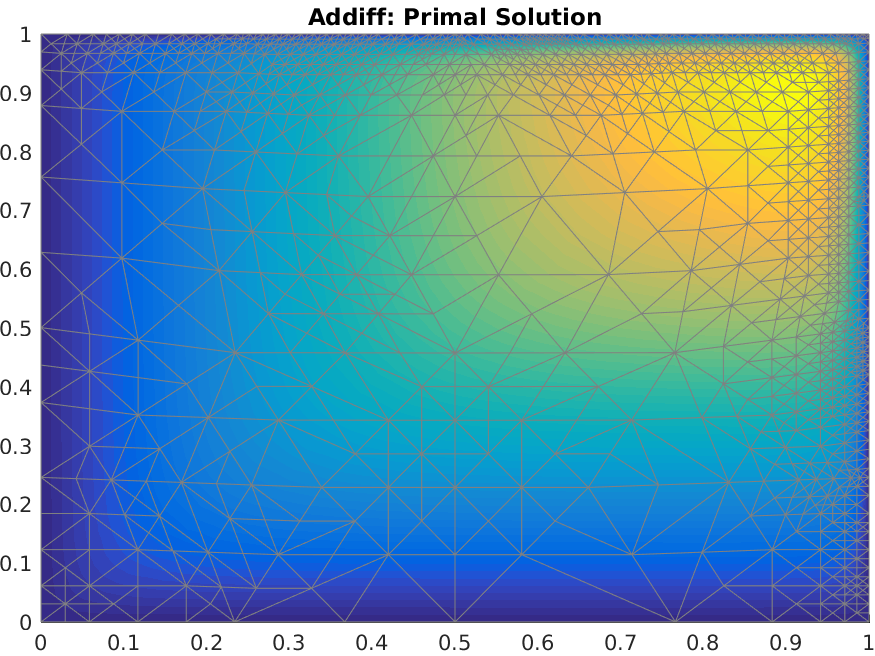
\includegraphics[width=0.8\textwidth]{addiff_primal_L2.pdf}
		\caption{Primal addiff solution with mesh, L2 Adapted}
		\label{fig:L2_primal}
	\end{figure}
	\begin{figure}[H]
		\centering
		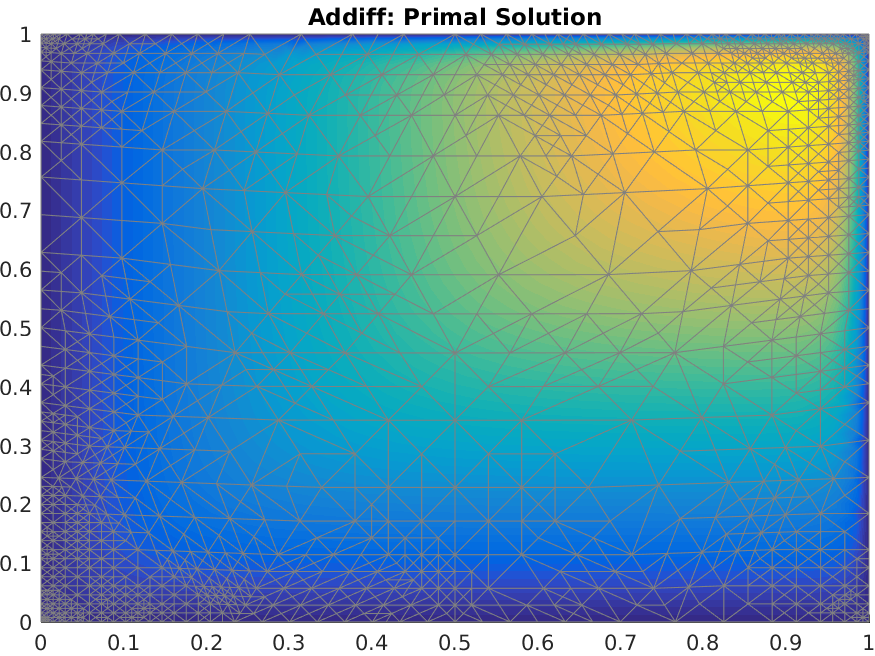
\includegraphics[width=0.8\textwidth]{addiff_primal.pdf}
		\caption{Primal addiff solution with mesh, Output Adapted}
		\label{fig:out_primal}
	\end{figure}
	
	We note that the adaptation driven by the error in the \(L^2\) norm of the solution adapts mostly in the top and right areas of the mesh. This can be expected as this is where the solution gradient is greatest. In the bottom and left regions the solution can be more accurately captured by a cheaper approximation.\\
	
	This can be constrasted with the output-based scheme; here it helps to look at the adjoint solution of the problem, as shown in Figure \ref{fig:out_adj} below.
	\begin{figure}[H]
		\centering
		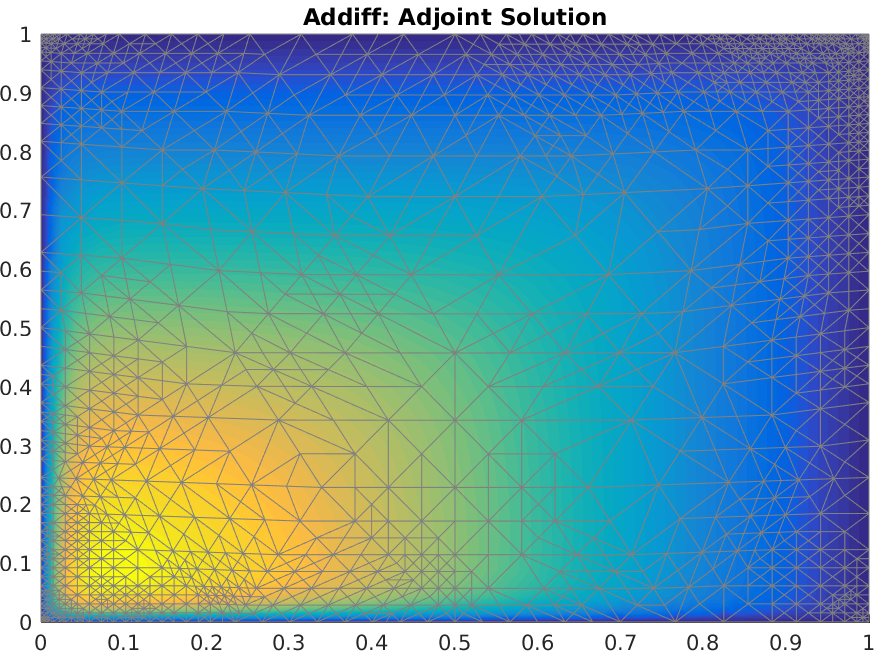
\includegraphics[width=0.8\textwidth]{addiff_adjoint.pdf}
		\caption{Adjoint solution with mesh, Output Adapted}
		\label{fig:out_adj}
	\end{figure}
	Here we note that when we weigh our indicators with the adjoint and primal solutions we obtain a more evenly distributed refinement strategy, with a slight preference to the edges of the domain. Again, we see that the gradient of the adjoint is greatest in the bottom left corner and the combination of this along with the primal error discussed previously is what yields the combined refinement strategy.
	


	
	Lastly, we plot the output error as a function of \(n\) for uniform, \(L^2\)-adaptive, and output-adaptive refinement in Figure \ref{Addiff:refinement} below. 
	\begin{figure}[H]
		\centering
		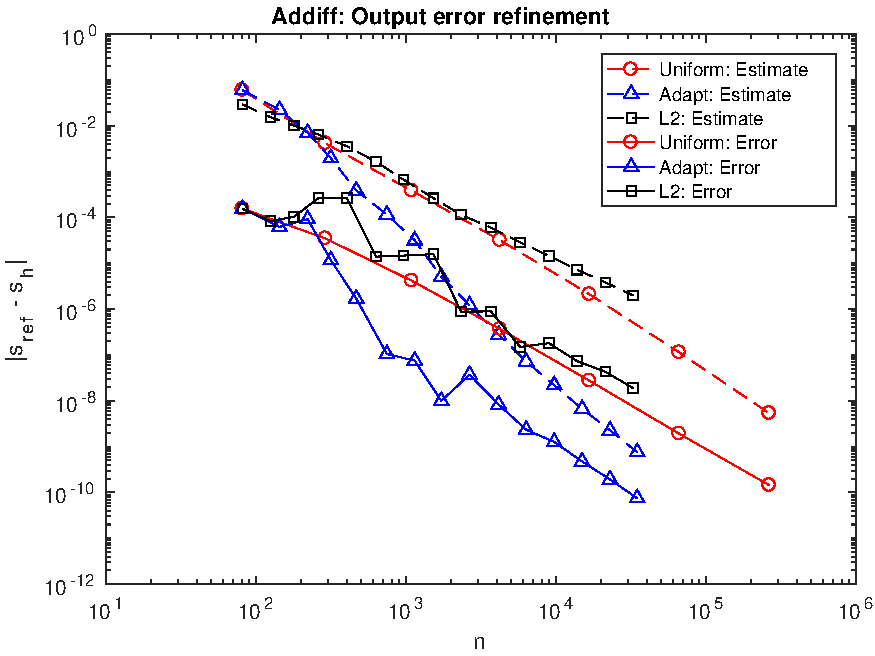
\includegraphics[width=0.8\textwidth]{addiff_adapt.pdf}
		\caption{Addiff refinemetn}
		\label{Addiff:refinement}
	\end{figure}
	The convergence rates are summarized in Table  \ref{tab:3} below.
	\begin{table}[H]
		\centering
		\begin{tabular}{r||c|c|c}
			& Uniform & \(L^2 \) & output  \\
			\hline
			Expected & -2.00 & -2.00 & -2.00\\
			\hline
			Actual &-2.2125  & -1.542 & -2.5700\\
		\end{tabular}
		\caption{Convergence rates for each of the adaptation algorithms}
		\label{tab:3}
	\end{table}
\end{itemize}
Here we see that the expected convergence rate of \(2p\) is in moderate agreement with the uniform and output-adaptive algorithms while the \(L^2\)-scheme falls slightly short. We can speculate that this is a result of the fact that the output error depends on both the error in the adjoint, and the \(L^2\) strategy will choose to refine only the error in the primal solution. This will cause the error in the adjoint to dominate while additional refinement is spent in areas of the domain that do not require it. 

\clearpage

\section*{Part 3. Adaptive eigensolver}
\begin{itemize}
	\item[(a)] The weak form of our eigenproblem on \(\Omega \equiv [0,1]^2 \) can be stated as: find \((u_k,\lambda_k) \in H^1_0(\Omega)\times \RR, k\in \ZZ_{>0} \) such that \(\|u_k\|_{L^2(\Omega)} \) and 
	\begin{equation*}
		\int_\Omega \nabla v \cdot \nabla u_k dx = \lambda_k \int_\Omega vu_kdx \quad \forall v \in H^1_0(\Omega).
	\end{equation*}
	Integrating by parts the left side of the  weak form of our eigenproblem above, we arrive at
	\begin{equation*}
		\int_{\partial\Omega} v(n\cdot\nabla u) ds - \int_\Omega v \nabla^2 u_k dx = \lambda_k \int_\Omega vu_kdx \quad \forall v \in H^1_0(\Omega),
	\end{equation*}
	a simple rearrangement yields
	\begin{equation*}
		\int_{\partial\Omega} v(n\cdot\nabla u) ds - \int_\Omega v(\nabla^2 u_k + \lambda_ku_k) dx = 0 \quad \forall v \in H^1_0(\Omega).
	\end{equation*}
	The strong form of the above is given by
	\begin{equation*}
		-\nabla^2u_k = \lambda_ku_k \text{ in } \Omega, \quad n\cdot\nabla u_k = 0 \text{ on } \partial\Omega.
	\end{equation*}
	This PDE is not separable but since it is in a form amenable to periodic solutions, let us guess the solution \(u_k = A_0\sin(k\pi x_1)\sin(k\pi x_2) \) --- \(A_0\) being some normalization constant --- and test our hypothesis. We note that 
	\begin{equation*}
		\nabla^2 u_k = 2k^2\pi^2u_k, \text{ and } n\cdot\nabla u_k = 0, \forall k\in\ZZ.
	\end{equation*}
	We note that since we require \(\|u_k\|_{L^2(\Omega)} = 1 \), and 
	\begin{equation*}
		\|u_k\|_{L^2(\Omega)} = \int_0^1\int_0^1 (\sin(k\pi x_1)\sin(k\pi x_2))^2 dx_1dx_2 = \dfrac{1}{4} \implies A_0 = 2,
	\end{equation*}
	our closed form expression for our first eigenpair on our unit-square domain is 
	\begin{equation*}
		(u_1, \lambda_1) = (2\sin(\pi x_1)\sin(\pi x_2), 2\pi^2).
	\end{equation*}
	
	\item[(b)] Let us define the eigenproblem on the arbitrary domain \(\tilde{\Omega} \) to be
	\begin{equation*}
		\int_{\tilde{\Omega}} \tilde{\nabla}v \cdot \tilde{\nabla}u_kd\tilde{x} = \tilde{\lambda_k}\int_{\tilde{\Omega}} v u_kd\tilde{x}.
	\end{equation*}
	We note that from the definition of our scaled domain \(\Omega \) we have 
	\begin{equation*}
		dx = Hd\tilde{x}, \implies \tilde{\nabla} = \pp{}{\tilde{x}} = \pp{}{x}\pp{x}{\tilde{x}} = H\nabla
	\end{equation*}
	This allows us to take our eingenproblem to be
	\begin{equation*}
		\int_{\Omega} H\nabla v \cdot H\nabla u_k\dfrac{dx}{H} = \tilde{\lambda_k}\int_{\Omega} v u_k\dfrac{dx}{H}.
	\end{equation*}
	\begin{equation*}
		\int_{\Omega} \nabla v \cdot \nabla u_k dx = \underbrace{\dfrac{\tilde{\lambda_k}}{H^2}}_{\lambda_k}\int_{\Omega} v u_k dx.
	\end{equation*}
	Here we notice that \(\lambda_k = \dfrac{\tilde{\lambda_k}}{H^2} \), and \(q = -2\). As a corolloray, we can note that \(\lambda_\text{min}^\text{S} = \dfrac{\lambda_1}{H^2} = \dfrac{\pi^2}{2} \)
	
	\item[(c)] We note that the smallest eigenvalue can be taken as a coercivity constant, i.e. the coercivity constant can be interpreted as the lower bound of the Rayleigh quotient, the lower bound of which is given by the smallest eigen value, expressed mathematically this says
	\begin{equation*}
		\lambda_\text{min} = \inf_k\{\lambda_k\} = \alpha = \inf\limits_{v\in\calV_h}\dfrac{a(v,v)}{\|v\|^2_{\calV_h}}.
	\end{equation*}
	Applying this to our L-shaped and square domains --- \(\Omega^\text{L}\) and \(\Omega^\text{S} \), respectively --- we obtain the following expressions
	\begin{equation*}
		\lambda_\text{min}^\text{S} = \inf\limits_{v\in H^1_0(\Omega^\text{S})}\dfrac{a^\text{S}(v,v)}{\|v\|^2_{H^1_0(\Omega^\text{S})}}, \quad \lambda_\text{min}^\text{L} = \inf\limits_{v\in H^1_0(\Omega^\text{L})}\dfrac{a^\text{L}(v,v)}{\|v\|^2_{H^1_0(\Omega^\text{L})}}.
	\end{equation*}
	Where \(a^\text{L}(v,v), a^\text{S}(v,v) \) are the bilinear form for the Rayleigh quatients on each space. We note that since we have \(H^1_0(\Omega^\text{L}) \subset H^1_0(\Omega^\text{S}) \) we can say that
	\begin{equation*}
		\lambda_\text{min}^\text{S} = \inf\limits_{v\in H^1_0(\Omega^\text{S})}\dfrac{a^\text{S}(v,v)}{\|v\|^2_{H^1_0(\Omega^\text{S})}} \leq   \inf\limits_{v\in H^1_0(\Omega^\text{L})}\dfrac{a^\text{L}(v,v)}{\|v\|^2_{H^1_0(\Omega^\text{L})}} = \lambda_\text{min}^\text{L}.
	\end{equation*}
	This demonstrates that \(\lambda_\text{min}^\text{S} \leq \lambda_\text{min}^\text{L} \).
	
	\item[(d)] We define \(\Omega^\text{U} \equiv [0,1]^2 \) to be the unit square and note that our square domain \(\Omega^\text{S} \)  can be expressed as
	\begin{equation*}
		\Omega^\text{S} = \{x\in\RR^2 : x = H\tilde{x} = 2\tilde{x}, \tilde{x} \in \Omega^\text{U} \}.
	\end{equation*}
	We note from part (a) that \(\lambda_\text{min}^U = \dfrac{\pi^2}{2} \), and that
	\begin{equation*}
		\lambda_\text{min}^S = H^{-2} \lambda_\text{min}^U = \dfrac{\pi^2}{2}.
	\end{equation*}
	Finally from part (c) we can say that
	\begin{equation*}
		\lambda_\text{min}^\text{S} \leq \lambda_\text{min}^\text{L} \implies \dfrac{\pi^2}{2} \leq \lambda_\text{min}^\text{L}.
	\end{equation*}
	Which is our upper bound for the smallest eigenvalue on the L-shaped domain.
	
	\item[(e-f)] See appendix.
	
	\item[(g)] A convergence plot for the \(L^2\) norm of the error in the first eigenfunction on the square domain is shown in Figure \ref{fig:eigsq_conv_1}.
	
	\begin{figure}[H]
		\centering
		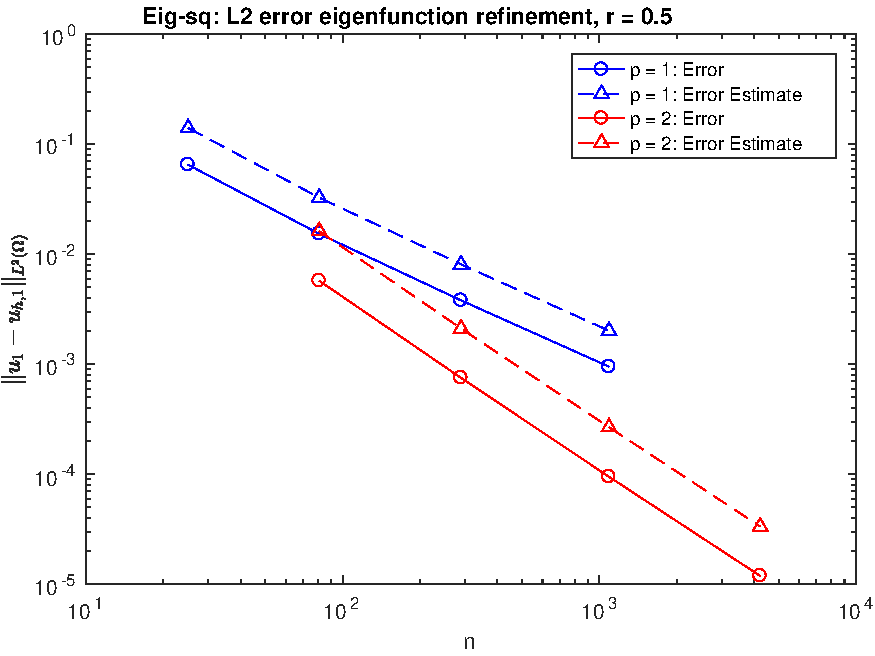
\includegraphics[width=0.8\textwidth]{eigsq_eigfun_adapt.pdf}
		\caption{Square domain first eigenfunction \(L^2\) norm convergence}
		\label{fig:eigsq_conv_1}
	\end{figure}
	Convergence rates for the \(L^2 \) norm of the error of the first eigenfunction are shown below in Table \ref{tab:31}, we note that they agree very well with the expected value of \((p+1)/2 \).
	\begin{table}[H]
		\centering
		\begin{tabular}{r||c|c}
			& \(\PP^1 \) & \(\PP^2 \) \\
			\hline
			Expected & -1.00 & -1.50 \\
			\hline
			Actual & -1.0253 & -1.5332 \\
		\end{tabular}
		\caption{Convergence rates for eigenfunction error on square domain}
		\label{tab:31}
	\end{table}
	When using a rate parameter of \(r = 1/2\) the effectivities for the \(\PP^1\) and \(\PP^2 \) schemes are \(\sim2.13 \) and \(\sim 2.82 \) respectively, both happen to be quite constant. Switching to \(r = 1\), the effectivities are still just as constant, but they are updated to become  \(\sim0.89 \) and \(\sim 1.16 \) for \(\PP^1\) and \(\PP^2 \) respectively.
	
	
	With regard to eigenvalues, their error as a function of \(n\) for uniform refinement are shown in Figure \ref{templabel2} below.
	\begin{figure}[H]
		\centering
		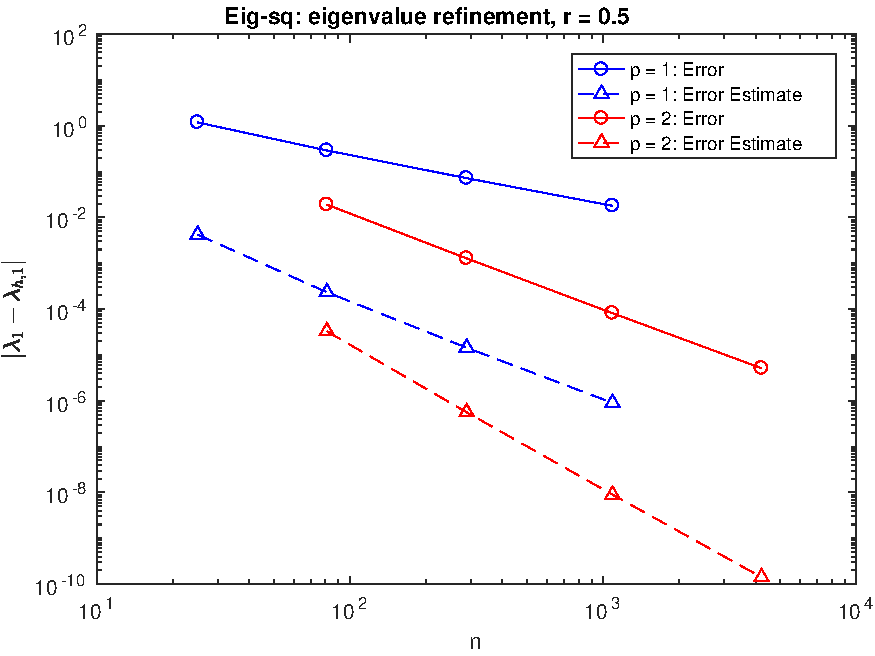
\includegraphics[width=0.8\textwidth]{eigsq_eigval_adapt.pdf}
		\caption{temp caption}
		\label{templabel2}
	\end{figure}
	Convergence rates for the above lines are shown in Table \ref{tab:32} below.
	\begin{table}[H]
		\centering
		\begin{tabular}{r||c|c}
			& \(\PP^1 \) & \(\PP^2 \) \\
			\hline
			Expected & -1.00 & -2.00 \\
			\hline
			Actual & -1.0492 & -2.0670 \\
		\end{tabular}
		\caption{Convergence rates for eigenvalue error on square domain}
		\label{tab:32}
	\end{table}
	Here it is clear that there is some scaling factor of error causing the large disagreement between the error and the error estimates. I'm not entirely sure what this is but the convergence rate is as expected for a functional output and the effectivities are quite constant.
	
	\item[(h)] The reference eigenvalue was found to be \(\lambda_1^\text{ref} =  9.639816656535080\) with an error estimate of \(1.702667539918248 \times 10^{-4} \), this was computed using 8 iterations of our adaptive algorithm. The resulting first eigenfunction \(u_1\) is shown in Figure \ref{fig:eigsl1}
	\begin{figure}[H]
		\centering
		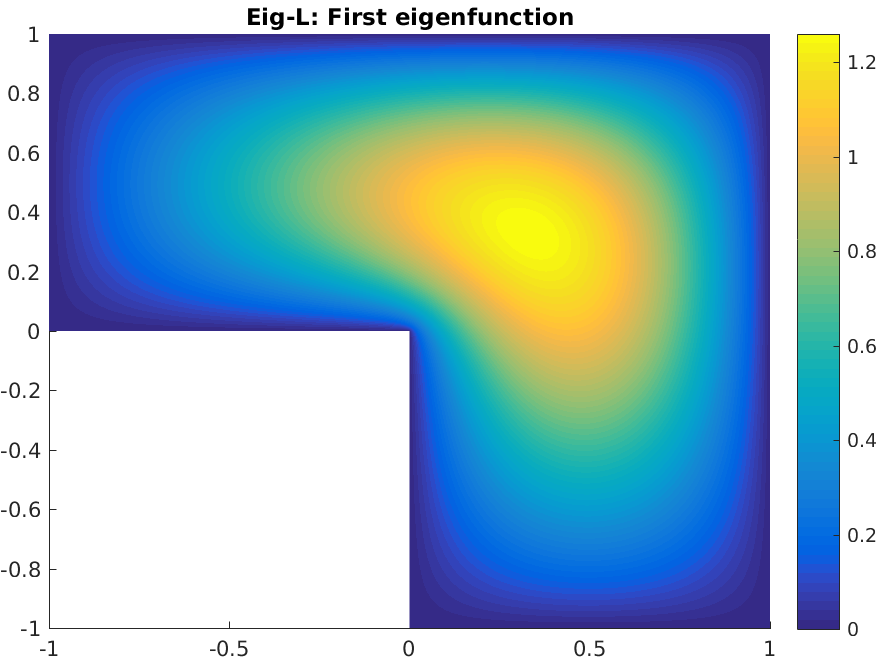
\includegraphics[width=0.8\textwidth]{eigl_eigfun.pdf}
		\caption{First eigenfunction on L-shaped membrane}
		\label{fig:eigsl1}
	\end{figure}
	
	\item[(h)] A convergence plot for the absolute value of the error in the first eigenvalue on the L-domain is shown in Figure \ref{fig:eigl_conv_1}.
	\begin{figure}[H]
		\centering
		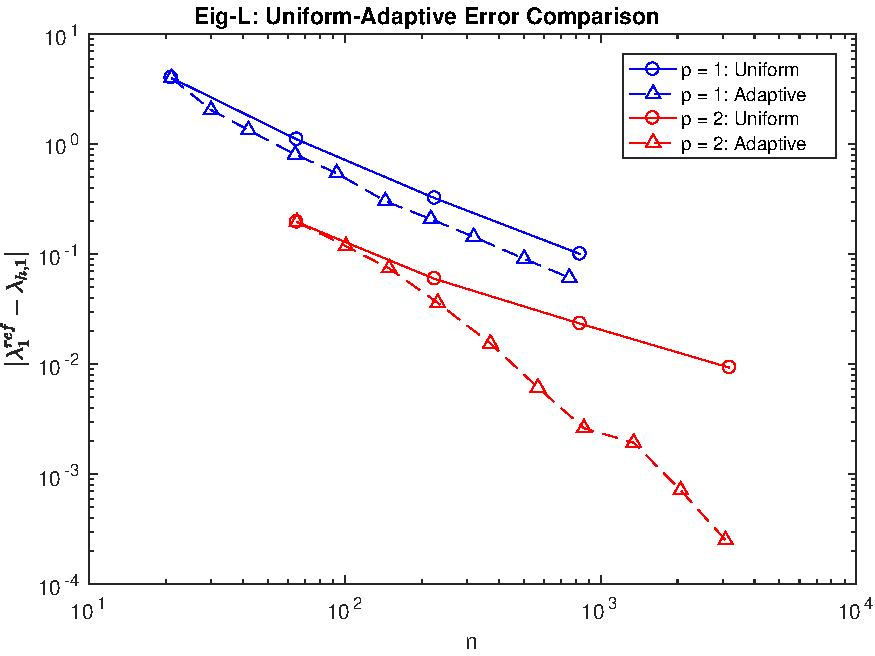
\includegraphics[width=0.8\textwidth]{eigl_conv_1.pdf}
		\caption{Square domain first eigenfunction \(L^2\) norm convergence}
		\label{fig:eigl_conv_1}
	\end{figure}
	Comparing uniform and adaptive refinement, we see evidence of a strong singularity in our domain. Where the uniform scheme cannot single out this region for more attention, the adaptive scheme does, and it allows us to achieve a higher convergence. These convergence rates are shown in Table \ref{tab:33} below. It further demonstrates that the convergence is highly limited by the regularity of the solution.
	
	\begin{table}[H]
		\centering
		\begin{tabular}{r||c|c}
			& \(\PP^1 \) & \(\PP^2 \) \\
			\hline
			Uniform & -0.8901 &  -0.6782 \\
			\hline
			Adaptive & -1.3375  & -2.1293 \\
		\end{tabular}
		\caption{Convergence rates for eigenvalue error on L domain}
		\label{tab:33}
	\end{table}
	
	A convergence plot (h)(iii) is shown in Figure \ref{fig:eigl_conv_2}.
	\begin{figure}[H]
		\centering
		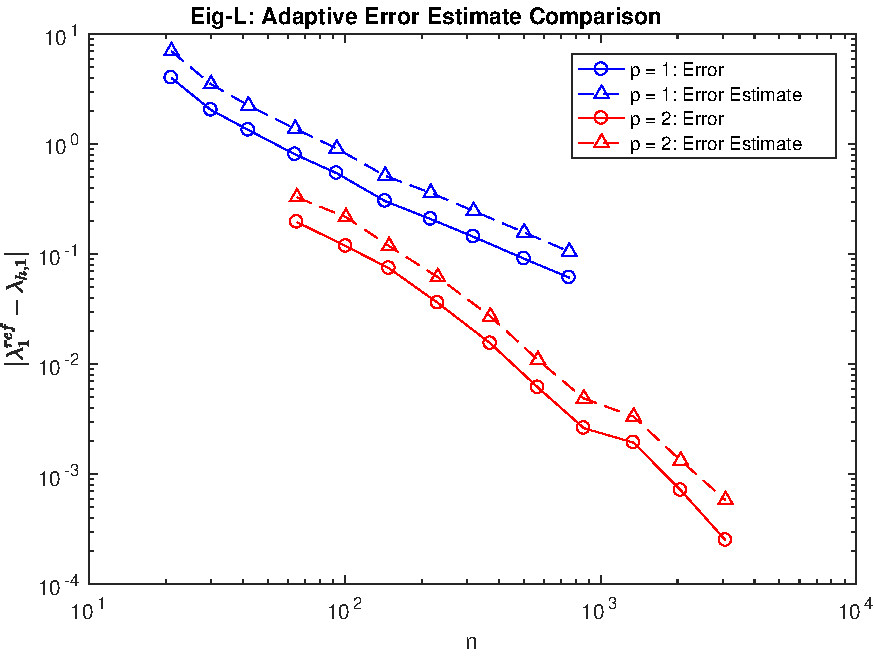
\includegraphics[width=0.8\textwidth]{eigl_conv_2.pdf}
		\caption{Square domain first eigenfunction \(L^2\) norm convergence}
		\label{fig:eigl_conv_2}
	\end{figure}
	The observed effectivity is comparable to that found for the square problem.
	
	
	Lastly, we consider the mesh for our L-shaped eigenfunction shown in Figure \ref{fig:eigl_soln}, it shows a strong singularity at the corner located at the origin. This explains our poorer convergence rates as compared with the square domain, and we also note that a large portion of the refinement has been located here. 
	\begin{figure}[H]
		\centering
		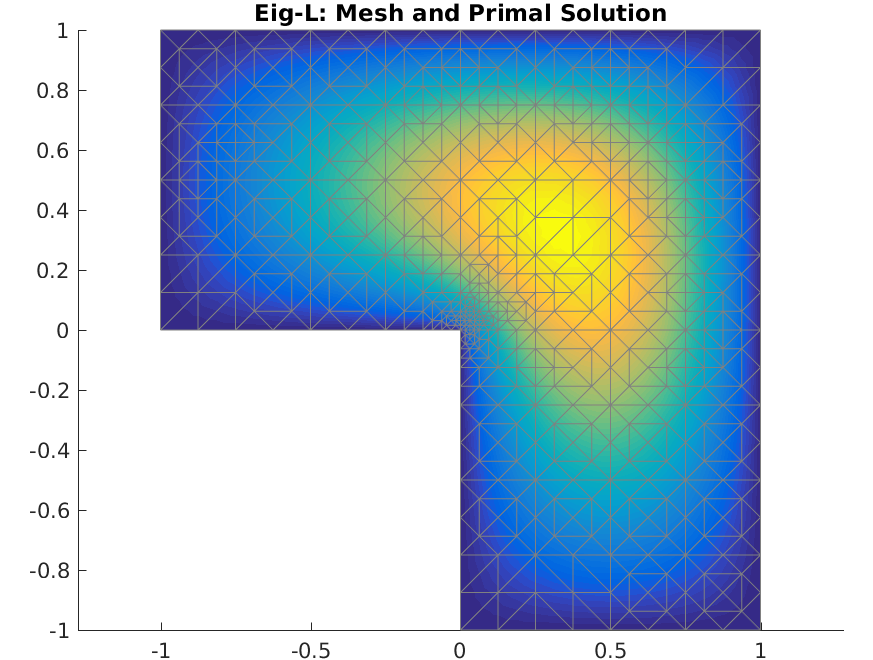
\includegraphics[width=0.8\textwidth]{eigl_mesh.pdf}
		\caption{Square domain first eigenfunction \(L^2\) norm convergence}
		\label{fig:eigl_soln}
	\end{figure}
	
	\item[(i)] This is the MathWorks logo.
	\begin{figure}[H]
		\centering
		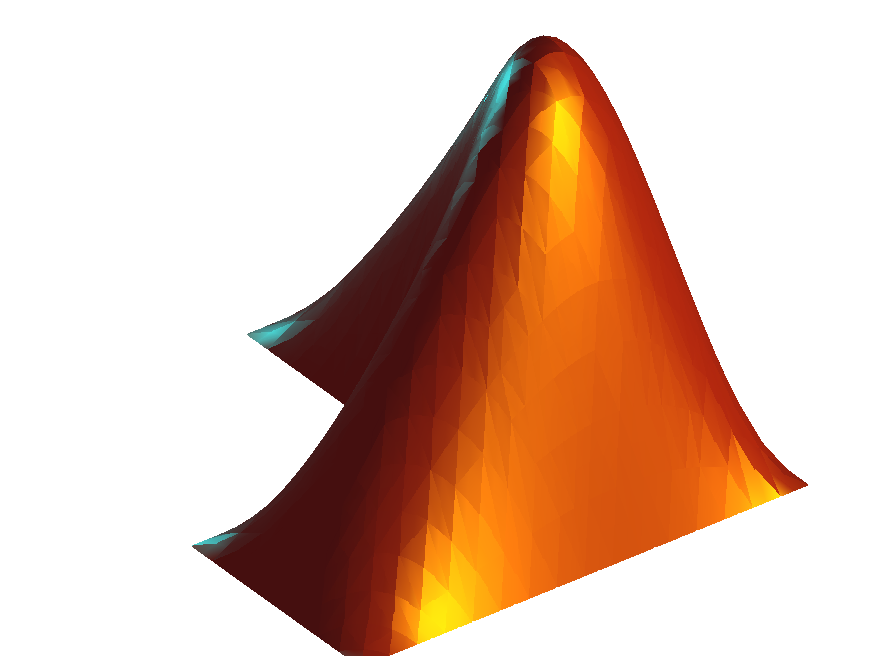
\includegraphics[width=0.8\textwidth]{matlab.pdf}
		\caption{First eigenfunction on L-shaped membrane}
	\end{figure}
\end{itemize}


\section*{Appendix}
\lstinputlisting[style=Matlab-editor]{../fem2d_part/ad_adapt_2d_template.m}
\end{document}
